\section{Asymmetric Fault Modeling}
\label{sec:byzantine}
A \textit{asymmetric} or \textit{Byzantine} fault is a fault that presents different symptoms to different observers~\cite{Driscoll-Byzantine-Fault}. In our modeling environment, asymmetric faults may be associated with a component that has a 1-n output to multiple other components. In this configuration, a \textit{symmetric} fault will result in all destination components seeing the same faulty value from the source component. To capture the behavior of asymmetric faults (``different symptoms to different observers''), it was necessary to extend our fault modeling mechanism in AADL. A thorough description of the asymmetric modeling capability of the Safety Annex is shown in Chapter~\ref{chap:caseStudies} using a process ID example.

\subsection{Implementation of Asymmetric Faults}
To illustrate our implementation of asymmetric faults, assume a source component A has a 1-n output connected to four destination components (B-E) as shown in Figure~\ref{fig:commNodes} under ``Nominal System.'' If a symmetric fault was present on this output, all four connected components would see the same faulty behavior. An asymmetric fault should be able to present arbitrarily different values to the connected components. 

To this end, ``communication nodes'' are inserted on each connection from component A to components B, C, D, and E (shown in Figure~\ref{fig:commNodes} under ``Fault Model Architecture.'' From the users perspective, the asymmetric fault definition is associated with component A's output and the architecture of the model is unchanged from the nominal model architecture. Behind the scenes, these communication nodes are created to facilitate potentially different fault activations on each of these connections. The fault definition used on the output of component A will be inserted into each of these communication nodes as shown by the red circles at the communication node output in Figure~\ref{fig:commNodes}.
\begin{figure}[!htb]
        \center{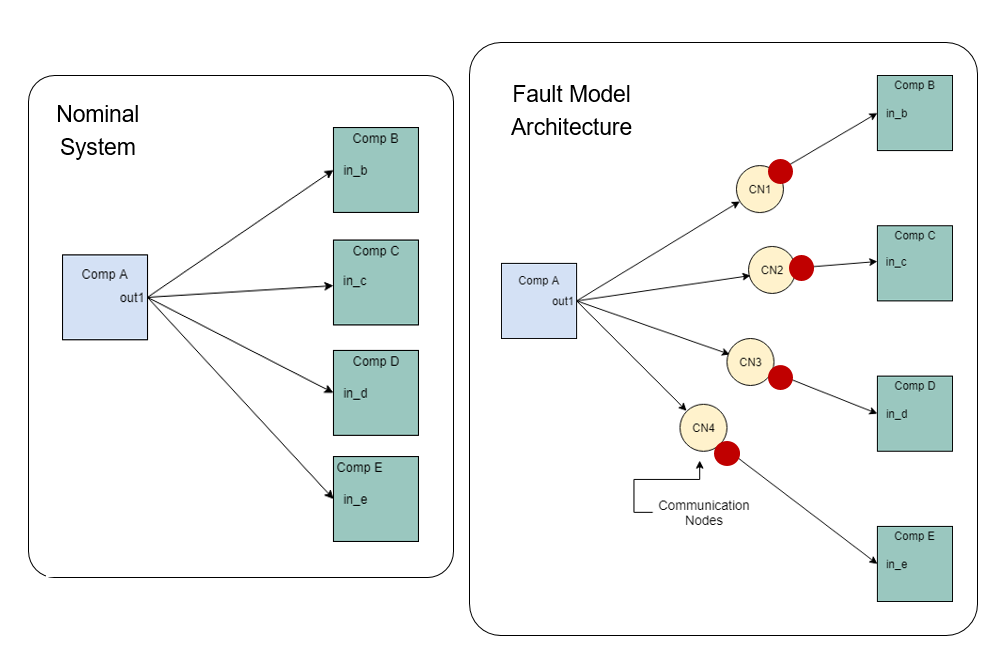
\includegraphics[width=\textwidth] {images/commNodes.png}}
        \caption{\label{fig:commNodes} Communication Nodes in Asymmetric Fault Implementation}
\end{figure}

\begin{figure}[!htb]
        \center{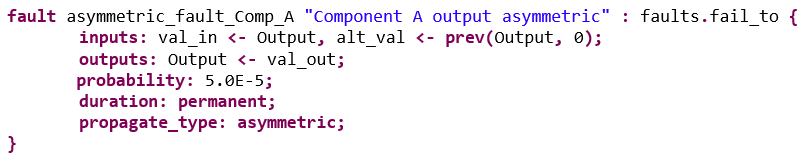
\includegraphics[width=\textwidth] {images/asymFaultDef.png}}
        \caption{\label{fig:asymFaultDef} Asymmetric Fault Definition in the Safety Annex}
\end{figure}

An asymmetric fault is defined for Component A as in Figure~\ref{fig:asymFaultDef}. This fault defines an asymmetric failure on Component A that when active, is stuck at a previous value (\textit{prev(Output, 0)}). This can be interpreted as the following: some connected components may only see the previous value of Comp A output and others may see the correct (current) value when the fault is active. This fault definition is injected into the communication nodes and which of the connected components see an incorrect value is completely nondeterministic. Any number of the communication node faults (0…all) may be active upon activation of the main asymmetric fault.

\subsection{Referencing Fault Activation Status}
To fully implement the agreement protocol, it must be possible to describe whether or not a subcomponent is failed by specifying if any faults defined for the subcomponents is activated. In the Safety Annex, this is made possible through the use of a \textit{fault activation} statement. Users can declare boolean \textit{eq} variables in the AGREE annex of the AADL system where the AGREE verification applies to that system's implementation. %in AGREE and in the implementations Safety Annex, 
Users can then assign the activation status of specific faults to those \textit{eq} variables in Safety Annex of the AADL system implementation (the same place where the fault analysis statement resides).
%assigns this boolean \textit{eq} statement to a fault specific to a subcomponent. 
This assignment links each specified AGREE boolean variable with the 
activation status of the specified fault activation literal. %It is 
The AGREE boolean variable is true when and only when the fault is active.

This additional feature of the Safety Annex allows users to state contracts of the form: if \texttt{sensor\_failed} then \texttt{do\_something}.

 

